%%%%%%%%%%%%%%%%%%%%%%%%%%%%%%%%%%%%%%%%%%%%%%%%%%%%%%%%%%%%%%%%%%
%%%%%%%% ICML 2016 EXAMPLE LATEX SUBMISSION FILE %%%%%%%%%%%%%%%%%
%%%%%%%%%%%%%%%%%%%%%%%%%%%%%%%%%%%%%%%%%%%%%%%%%%%%%%%%%%%%%%%%%%

% Use the following line _only_ if you're still using LaTeX 2.09.
%\documentstyle[icml2016,epsf,natbib]{article}
% If you rely on Latex2e packages, like most moden people use this:
\documentclass{article}

% use Times
\usepackage{times}
% For figures
\usepackage{graphicx} % more modern
%\usepackage{epsfig} % less modern
\usepackage{subfigure} 

% For citations
\usepackage{natbib}

% For algorithms
\usepackage{algorithm}
\usepackage{algorithmic}

% As of 2011, we use the hyperref package to produce hyperlinks in the
% resulting PDF.  If this breaks your system, please commend out the
% following usepackage line and replace \usepackage{icml2016} with
% \usepackage[nohyperref]{icml2016} above.
\usepackage{hyperref}

% Packages hyperref and algorithmic misbehave sometimes.  We can fix
% this with the following command.
\newcommand{\theHalgorithm}{\arabic{algorithm}}

% Employ the following version of the ``usepackage'' statement for
% submitting the draft version of the paper for review.  This will set
% the note in the first column to ``Under review.  Do not distribute.''
\usepackage[accepted]{icml2016} 

%\usepackage{icml_numpapers}


% The \icmltitle you define below is probably too long as a header.
% Therefore, a short form for the running title is supplied here:
\icmltitlerunning{ORIE 6741 Project Proposal 10/27/2017}

\begin{document} 

\twocolumn[
\icmltitle{Title (10/27/2017)}

% It is OKAY to include author information, even for blind
% submissions: the style file will automatically remove it for you
% unless you've provided the [accepted] option to the icml2016
% package.
\icmlauthor{name}{email@domain.edu}
\icmladdress{netid}
\icmlauthor{name}{email@domain.edu}
\icmladdress{netid}
\icmlauthor{name}{email@domain.edu}
\icmladdress{netid}


% You may provide any keywords that you 
% find helpful for describing your paper; these are used to populate 
% the "keywords" metadata in the PDF but will not be shown in the document
\icmlkeywords{boring formatting information, machine learning, ICML}

\vskip 0.3in
]

\begin{abstract} 
The purpose of this document is to provide both the basic paper template and
submission guidelines. Abstracts should be a single paragraph, between 4--6 sentences long, ideally.  Gross violations will trigger corrections at the camera-ready phase.
\end{abstract} 

\section{Motivation}
Time series data in several domains is highly volatile and difficult to predict. One crucial reason is the presence of change point -- a drastic change in the response due to several potential reasons including seasonality, marketing intervention , natural disaster or panic. Without incorporating change point into the model, the accuracy of the model can be severely affected. Another challenge is to automatically predict when the change point is going to happen. An agent that can automatically locate change point in real time and use the information to adjust the prediction can result in a fully automated monitoring system and real time prediction system. Most of the change point detection algorithm is frequentist model which is not fully data-driven. Here we will use Bayesian method with MCMC to detect change points and Gaussian Process to do extrapolation.

\section{Format of the Paper} 
 
All submissions must follow the same format to ensure the printer can
reproduce them without problems and to let readers more easily find
the information that they desire.

\subsection{Length and Dimensions}

Papers must not exceed eight (8) pages, including all figures, tables,
and appendices, but excluding references and acknowledgements. When references and acknowledgements are included,
the paper must not exceed ten (10) pages.
Acknowledgements should be limited to grants and people who contributed to the paper.
Any submission that exceeds 
this page limit or that diverges significantly from the format specified 
herein will be rejected without review.

The text of the paper should be formatted in two columns, with an
overall width of 6.75 inches, height of 9.0 inches, and 0.25 inches
between the columns. The left margin should be 0.75 inches and the top
margin 1.0 inch (2.54~cm). The right and bottom margins will depend on
whether you print on US letter or A4 paper, but all final versions
must be produced for US letter size.

The paper body should be set in 10~point type with a vertical spacing
of 11~points. Please use Times typeface throughout the text.

\subsection{Title}

The paper title should be set in 14~point bold type and centered
between two horizontal rules that are 1~point thick, with 1.0~inch
between the top rule and the top edge of the page. Capitalize the
first letter of content words and put the rest of the title in lower
case.

\subsection{Author Information for Submission}
\label{author info}

To facilitate blind review, author information must not appear.  If
you are using \LaTeX\/ and the \texttt{icml2016.sty} file, you may use
\verb+\icmlauthor{...}+ to specify authors.  The author information
will simply not be printed until {\tt accepted} is an argument to the
style file. Submissions that include the author information will not
be reviewed.

\subsubsection{Self-Citations}

If your are citing published papers for which you are an author, refer
to yourself in the third person. In particular, do not use phrases
that reveal your identity (e.g., ``in previous work \cite{langley00}, we 
have shown \ldots'').

Do not anonymize citations in the reference section by removing or
blacking out author names. The only exception are manuscripts that are
not yet published (e.g. under submission). If you choose to refer to
such unpublished manuscripts \cite{anonymous}, anonymized copies have 
to be submitted
as Supplementary Material via CMT. However, keep in mind that an ICML
paper should be self contained and should contain sufficient detail
for the reviewers to evaluate the work. In particular, reviewers are
not required to look a the Supplementary Material when writing their
review.

\subsubsection{Camera-Ready Author Information}
\label{final author}

If a paper is accepted, a final camera-ready copy must be prepared.
%
For camera-ready papers, author information should start 0.3~inches
below the bottom rule surrounding the title. The authors' names should
appear in 10~point bold type, electronic mail addresses in 10~point
small capitals, and physical addresses in ordinary 10~point type.
Each author's name should be flush left, whereas the email address
should be flush right on the same line. The author's physical address
should appear flush left on the ensuing line, on a single line if
possible. If successive authors have the same affiliation, then give
their physical address only once.

A sample file (in PDF) with author names is included in the ICML2016 
style file package.

\subsection{Abstract}

The paper abstract should begin in the left column, 0.4~inches below
the final address. The heading `Abstract' should be centered, bold,
and in 11~point type. The abstract body should use 10~point type, with
a vertical spacing of 11~points, and should be indented 0.25~inches
more than normal on left-hand and right-hand margins. Insert
0.4~inches of blank space after the body. Keep your abstract brief and 
self-contained,
limiting it to one paragraph and roughly 4--6 sentences.  Gross violations will require correction at the camera-ready phase.

\subsection{Partitioning the Text} 

You should organize your paper into sections and paragraphs to help
readers place a structure on the material and understand its
contributions.

\subsubsection{Sections and Subsections}

Section headings should be numbered, flush left, and set in 11~pt bold
type with the content words capitalized. Leave 0.25~inches of space
before the heading and 0.15~inches after the heading.

Similarly, subsection headings should be numbered, flush left, and set
in 10~pt bold type with the content words capitalized. Leave
0.2~inches of space before the heading and 0.13~inches afterward.

Finally, subsubsection headings should be numbered, flush left, and
set in 10~pt small caps with the content words capitalized. Leave
0.18~inches of space before the heading and 0.1~inches after the
heading. 

Please use no more than three levels of headings.

\subsubsection{Paragraphs and Footnotes}

Within each section or subsection, you should further partition the
paper into paragraphs. Do not indent the first line of a given
paragraph, but insert a blank line between succeeding ones.
 
You can use footnotes\footnote{For the sake of readability, footnotes
should be complete sentences.} to provide readers with additional
information about a topic without interrupting the flow of the paper. 
Indicate footnotes with a number in the text where the point is most
relevant. Place the footnote in 9~point type at the bottom of the
column in which it appears. Precede the first footnote in a column
with a horizontal rule of 0.8~inches.\footnote{Multiple footnotes can
appear in each column, in the same order as they appear in the text,
but spread them across columns and pages if possible.}

\begin{figure}[ht]
\vskip 0.2in
\begin{center}
\centerline{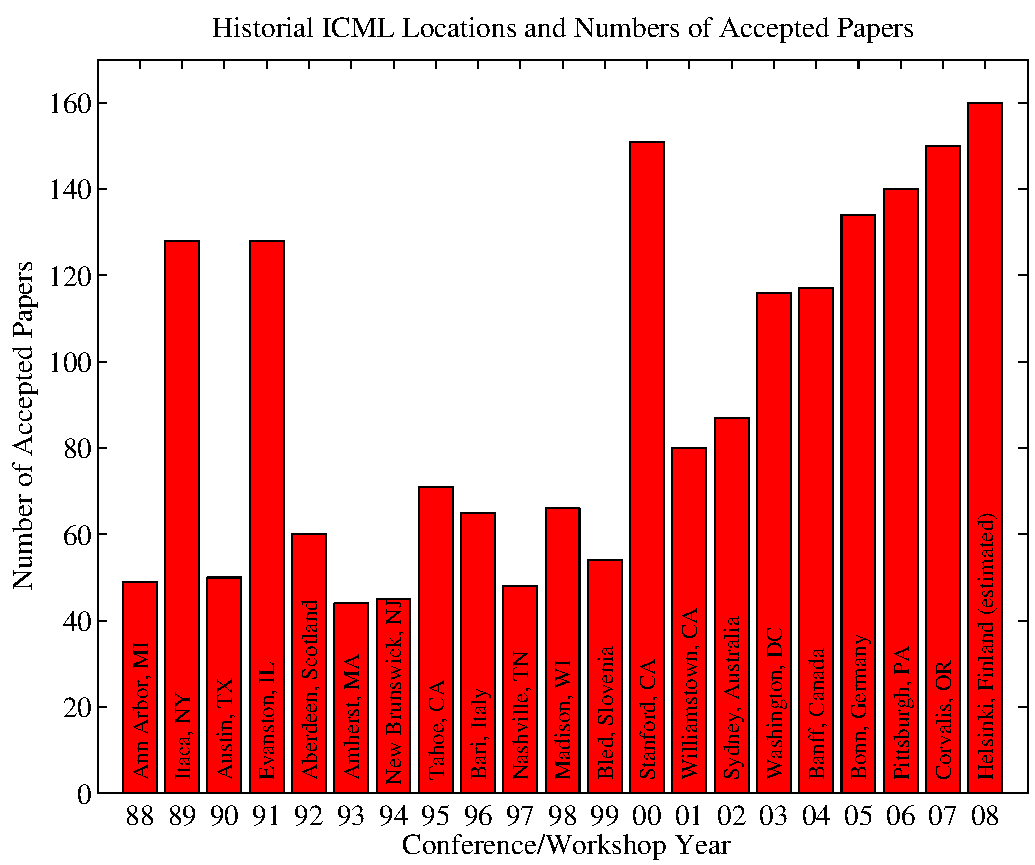
\includegraphics[width=\columnwidth]{icml_numpapers}}
\caption{Historical locations and number of accepted papers for International
  Machine Learning Conferences (ICML 1993 -- ICML 2008) and
  International Workshops on Machine Learning (ML 1988 -- ML
  1992). At the time this figure was produced, the number of
  accepted papers for ICML 2008 was unknown and instead estimated.}
\label{icml-historical}
\end{center}
\vskip -0.2in
\end{figure} 

\subsection{Figures}
 
You may want to include figures in the paper to help readers visualize
your approach and your results. Such artwork should be centered,
legible, and separated from the text. Lines should be dark and at
least 0.5~points thick for purposes of reproduction, and text should
not appear on a gray background.

Label all distinct components of each figure. If the figure takes the
form of a graph, then give a name for each axis and include a legend
that briefly describes each curve. Do not include a title inside the
figure; instead, the caption should serve this function.

Number figures sequentially, placing the figure number and caption
{\it after\/} the graphics, with at least 0.1~inches of space before
the caption and 0.1~inches after it, as in
Figure~\ref{icml-historical}.  The figure caption should be set in
9~point type and centered unless it runs two or more lines, in which
case it should be flush left.  You may float figures to the top or
bottom of a column, and you may set wide figures across both columns
(use the environment {\tt figure*} in \LaTeX), but always place
two-column figures at the top or bottom of the page.

\subsection{Algorithms}

If you are using \LaTeX, please use the ``algorithm'' and ``algorithmic'' 
environments to format pseudocode. These require 
the corresponding stylefiles, algorithm.sty and 
algorithmic.sty, which are supplied with this package. 
Algorithm~\ref{alg:example} shows an example. 

\begin{algorithm}[tb]
   \caption{Bubble Sort}
   \label{alg:example}
\begin{algorithmic}
   \STATE {\bfseries Input:} data $x_i$, size $m$
   \REPEAT
   \STATE Initialize $noChange = true$.
   \FOR{$i=1$ {\bfseries to} $m-1$}
   \IF{$x_i > x_{i+1}$} 
   \STATE Swap $x_i$ and $x_{i+1}$
   \STATE $noChange = false$
   \ENDIF
   \ENDFOR
   \UNTIL{$noChange$ is $true$}
\end{algorithmic}
\end{algorithm}


% Note use of \abovespace and \belowspace to get reasonable spacing 
% above and below tabular lines. 


Tables contain textual material that can be typeset, as contrasted 
with figures, which contain graphical material that must be drawn. 
Specify the contents of each row and column in the table's topmost
row. Again, you may float tables to a column's top or bottom, and set
wide tables across both columns, but place two-column tables at the
top or bottom of the page.
 
\subsection{Citations and References} 

Please use APA reference format regardless of your formatter
or word processor. If you rely on the \LaTeX\/ bibliographic 
facility, use {\tt natbib.sty} and {\tt icml2016.bst} 
included in the style-file package to obtain this format.

Citations within the text should include the authors' last names and
year. If the authors' names are included in the sentence, place only
the year in parentheses, for example when referencing Arthur Samuel's
pioneering work \yrcite{Samuel59}. Otherwise place the entire
reference in parentheses with the authors and year separated by a
comma \cite{Samuel59}. List multiple references separated by
semicolons \cite{kearns89,Samuel59,mitchell80}. Use the `et~al.'
construct only for citations with three or more authors or after
listing all authors to a publication in an earlier reference \cite{MachineLearningI}.

Authors should cite their own work in the third person
in the initial version of their paper submitted for blind review.
Please refer to Section~\ref{author info} for detailed instructions on how to
cite your own papers.

Use an unnumbered first-level section heading for the references, and 
use a hanging indent style, with the first line of the reference flush
against the left margin and subsequent lines indented by 10 points. 
The references at the end of this document give examples for journal
articles \cite{Samuel59}, conference publications \cite{langley00}, book chapters \cite{Newell81}, books \cite{DudaHart2nd}, edited volumes \cite{MachineLearningI}, 
technical reports \cite{mitchell80}, and dissertations \cite{kearns89}. 

Alphabetize references by the surnames of the first authors, with
single author entries preceding multiple author entries. Order
references for the same authors by year of publication, with the
earliest first. Make sure that each reference includes all relevant
information (e.g., page numbers).



% In the unusual situation where you want a paper to appear in the
% references without citing it in the main text, use \nocite
\nocite{langley00}

\bibliography{example_paper}
\bibliographystyle{icml2016}

\end{document} 


% This document was modified from the file originally made available by
% Pat Langley and Andrea Danyluk for ICML-2K. This version was
% created by Lise Getoor and Tobias Scheffer, it was slightly modified  
% from the 2010 version by Thorsten Joachims & Johannes Fuernkranz, 
% slightly modified from the 2009 version by Kiri Wagstaff and 
% Sam Roweis's 2008 version, which is slightly modified from 
% Prasad Tadepalli's 2007 version which is a lightly 
% changed version of the previous year's version by Andrew Moore, 
% which was in turn edited from those of Kristian Kersting and 
% Codrina Lauth. Alex Smola contributed to the algorithmic style files.  
